% ============================================================
%  يُترجَم بـ XeLaTeX  (في Overleaf: Menu → Compiler → XeLaTeX)
%  الخط: Amiri (متوفر في Overleaf، أو حمّله من github.com/aliftype/amiri)
% ============================================================
\documentclass[12pt,a4paper]{article}
\usepackage[a4paper,margin=1.7cm,top=2.3cm,bottom=2.9cm,headheight=15pt,footskip=1.5cm]{geometry}
\usepackage{amsmath,amssymb}
\usepackage{icomma}
\usepackage[english,bidi=default,layout=lists]{babel}
\babelprovide[import,main]{arabic}
\babelfont{rm}[Scale=1.08]{Amiri}
\babelfont{sf}[Scale=1.08]{Amiri}
\usepackage[most]{tcolorbox}
\usepackage{tikz}
\usetikzlibrary{arrows.meta,calc,shadings}
\usepackage{array}
\usepackage{colortbl}
\usepackage{fancyhdr}
\usepackage{titlesec}
\usepackage{enumitem}
\usepackage{collcell}
\usepackage{needspace}
\usepackage{etoolbox}
\newcolumntype{C}{>{\collectcell\ar}c<{\endcollectcell}}
\pretocmd{\section}{\Needspace{15\baselineskip}}{}{}
\pretocmd{\subsection}{\Needspace{11\baselineskip}}{}{}

\definecolor{cDef}{HTML}{1F4E9C}
\definecolor{cThm}{HTML}{B3261E}
\definecolor{cRem}{HTML}{2E7D32}
\definecolor{cEx}{HTML}{C76B00}
\definecolor{cMeth}{HTML}{6A1B9A}
\definecolor{cSol}{HTML}{00695C}
\definecolor{cSec}{HTML}{1F3A68}

\titleformat{\section}{\Large\bfseries\color{cSec}}{\thesection.}{0.6em}{}[{\color{cSec!60}\titlerule[1pt]}]
\titleformat{\subsection}{\large\bfseries\color{cThm!85!black}}{\thesubsection.}{0.5em}{}
\titlespacing*{\section}{0pt}{14pt}{8pt}
\titlespacing*{\subsection}{0pt}{10pt}{5pt}
\setlength{\parindent}{0pt}
\setlength{\parskip}{4pt}
\setlist{itemsep=2pt,topsep=3pt}

\newtcolorbox{arbox}[3][]{enhanced,
  colback=#2!5,colframe=#2!80!black,arc=2mm,boxrule=0.8pt,
  left=6pt,right=6pt,top=8pt,bottom=5pt,
  fonttitle=\bfseries,coltitle=white,
  title={\foreignlanguage{arabic}{#3}},
  attach boxed title to top right={xshift=-5mm,yshift=-3mm},
  boxed title style={colback=#2!80!black,arc=1.5mm,boxrule=0pt},
  before upper={\selectlanguage{arabic}},
  before skip=8pt,after skip=8pt,breakable,#1}
\newenvironment{BOX}[2]{\begin{otherlanguage}{english}\begin{arbox}{#1}{#2}}{\end{arbox}\end{otherlanguage}}
\newenvironment{tarif}[1][تعريف]{\begin{BOX}{cDef}{#1}}{\end{BOX}}
\newenvironment{khassia}[1][خاصية]{\begin{BOX}{cThm}{#1}}{\end{BOX}}
\newenvironment{molahada}[1][ملاحظة]{\begin{BOX}{cRem}{#1}}{\end{BOX}}
\newenvironment{mithal}[1][مثال]{\begin{BOX}{cEx}{#1}}{\end{BOX}}
\newenvironment{tariqa}[1][طريقة]{\begin{BOX}{cMeth}{#1}}{\end{BOX}}

\newcounter{exo}
\newenvironment{tamrin}[1]{\stepcounter{exo}\begin{BOX}{cSec}{التمرين \theexo: #1}}{\end{BOX}}
\newenvironment{hal}{\Needspace{12\baselineskip}\begin{otherlanguage}{english}\begin{arbox}[breakable]{cSol}{حل التمرين \theexo}}{\end{arbox}\end{otherlanguage}}

\newenvironment{LTR}{\begin{otherlanguage}{english}}{\end{otherlanguage}}
\newcommand{\ar}[1]{\foreignlanguage{arabic}{#1}}

\renewcommand{\dots}{\mathinner{\ldotp\ldotp\ldotp}}
\renewcommand{\ldots}{\mathinner{\ldotp\ldotp\ldotp}}
\renewcommand{\cdots}{\mathinner{\cdotp\cdotp\cdotp}}
\newcommand{\N}{\mathbb{N}}
\newcommand{\Z}{\mathbb{Z}}
\newcommand{\D}{\mathbb{D}}
\newcommand{\Q}{\mathbb{Q}}
\newcommand{\R}{\mathbb{R}}
\newcommand{\pgcd}{\operatorname{PGCD}}
\newcommand{\ppcm}{\operatorname{PPCM}}

% \NLseg{a}{b}{[}{]} ; \NLright{a}{[} ; \NLleft{b}{]}  (interval on a number line)
\newcommand{\NLseg}[4]{\begin{LTR}\begin{tikzpicture}[baseline=-0.6ex]
 \draw[-{Stealth[length=2mm]},gray!70](0,0)--(3.4,0);
 \draw[line width=2pt,cThm!80!black](0.7,0)--(2.7,0);
 \node[cThm!80!black,font=\LARGE] at (0.7,0){$#3$};
 \node[cThm!80!black,font=\LARGE] at (2.7,0){$#4$};
 \node[below=3pt,font=\footnotesize] at (0.7,0){$#1$};
 \node[below=3pt,font=\footnotesize] at (2.7,0){$#2$};
\end{tikzpicture}\end{LTR}}
\newcommand{\NLright}[2]{\begin{LTR}\begin{tikzpicture}[baseline=-0.6ex]
 \draw[-{Stealth[length=2mm]},gray!70](0,0)--(3.4,0);
 \draw[line width=2pt,cThm!80!black](1.3,0)--(3.3,0);
 \node[cThm!80!black,font=\LARGE] at (1.3,0){$#2$};
 \node[below=3pt,font=\footnotesize] at (1.3,0){$#1$};
\end{tikzpicture}\end{LTR}}
\newcommand{\NLleft}[2]{\begin{LTR}\begin{tikzpicture}[baseline=-0.6ex]
 \draw[-{Stealth[length=2mm]},gray!70](0,0)--(3.4,0);
 \draw[line width=2pt,cThm!80!black](0.05,0)--(2.1,0);
 \node[cThm!80!black,font=\LARGE] at (2.1,0){$#2$};
 \node[below=3pt,font=\footnotesize] at (2.1,0){$#1$};
\end{tikzpicture}\end{LTR}}

% ---------- social-media icons (pure TikZ) ----------
\definecolor{cFB}{HTML}{1877F2}
\definecolor{cTG}{HTML}{229ED9}
\definecolor{cIG1}{HTML}{FEDA75}
\definecolor{cIG2}{HTML}{D62976}
\definecolor{cIG3}{HTML}{4F5BD5}
\newcommand{\fbicon}{\begin{LTR}\begin{tikzpicture}[baseline=-0.75ex,x=1em,y=1em]
 \fill[cFB] (0,0) circle (0.55);
 \node[white,inner sep=0,font=\usefont{TU}{lmss}{bx}{n}\small] at (0.04,-0.02) {f};
\end{tikzpicture}\end{LTR}}
\newcommand{\igicon}{\begin{LTR}
\begin{tikzpicture}[baseline=-0.75ex,x=1em,y=1em]
 \shade[lower left=cIG1,lower right=cIG2,upper left=cIG2,upper right=cIG3,rounded corners=0.28em] (-0.55,-0.55) rectangle (0.55,0.55);
 \draw[white,line width=0.09em,rounded corners=0.18em] (-0.36,-0.36) rectangle (0.36,0.36);
 \draw[white,line width=0.09em] (0,0) circle (0.17);
 \fill[white] (0.22,0.22) circle (0.05);
\end{tikzpicture}\end{LTR}}
\newcommand{\tgicon}{\begin{LTR}
\begin{tikzpicture}[baseline=-0.75ex,x=1em,y=1em]
 \fill[cTG] (0,0) circle (0.55);
 \fill[white] (-0.33,0.0) -- (0.32,0.27) -- (0.2,-0.3) -- (0.0,-0.15) -- (-0.08,-0.28) -- (-0.08,-0.08) -- cycle;
 \fill[cTG!70!black] (-0.08,-0.08) -- (0.25,0.2) -- (0.0,-0.15) -- (-0.08,-0.28) -- cycle;
\end{tikzpicture}\end{LTR}}
% page number: black box, white two-digit number, at the right of the social row
\newcommand{\PageBox}{\begin{LTR}\tikz[baseline=(p.base)]\node[fill=black,text=white,inner sep=2.5pt,minimum width=1.6em,minimum height=1.3em,font=\usefont{TU}{lmss}{bx}{n}\small](p){\ifnum\value{page}<10 0\fi\arabic{page}};\end{LTR}}
% visual left-to-right order: Telegram | Instagram | Facebook | page box
\newcommand{\SocialRow}{\begin{otherlanguage}{english}%
 \ar{\textbf{الأستاذ سوايسية هشام للرياضيات}}\ \tgicon\hfill
 \textbf{prof\_hicham\_math}\ \igicon\hfill
 \ar{\textbf{الأستاذ سوايسية هشام للرياضيات}}\ \fbicon\hspace{2.2em}\PageBox\end{otherlanguage}}

\pagestyle{fancy}
\fancyhf{}
\renewcommand{\headrulewidth}{0.6pt}
\renewcommand{\footrulewidth}{0.4pt}
% \SetHeader{right head: document title}{left head: level -- stream}
\newcommand{\SetHeader}[2]{%
 \fancyhead[C]{\parbox{\textwidth}{\ar{#1\hfill #2}}}%
 \fancyfoot[C]{\parbox{\textwidth}{\small\SocialRow}}}
\usepackage{tkz-tab}
\usepackage{multicol}
% variation / sign table (LTR)
\newenvironment{TAB}{\par\begin{center}\begin{LTR}\begin{tikzpicture}[scale=0.95,every node/.style={font=\small}]}{\end{tikzpicture}\end{LTR}\end{center}}
% grid + axes, clipped: \begin{GR}{xmin}{xmax}{ymin}{ymax}{unit cm}
\newenvironment{GR}[5]{\par\begin{center}\begin{LTR}\begin{tikzpicture}[x=#5cm,y=#5cm,font=\footnotesize]
 \draw[gray!25,very thin] (#1,#3) grid (#2,#4);
 \draw[-{Stealth[length=2mm]}] (#1,0)--(#2+0.3,0) node[below left]{$x$};
 \draw[-{Stealth[length=2mm]}] (0,#3)--(0,#4+0.3) node[below left]{$y$};
 \node[below left] at (0,0){$O$};
 \begin{scope}\clip (#1,#3) rectangle (#2,#4);}
{\end{scope}\end{tikzpicture}\end{LTR}\end{center}}
\newcommand{\Ticks}[2]{\foreach \t in {#1} \node[below,font=\scriptsize] at (\t,0){$\t$}; \foreach \t in {#2} \node[left,font=\scriptsize] at (0,\t){$\t$};}
\newcommand{\bx}[1]{\ensuremath{\colorbox{cDef!12}{$\displaystyle #1$}}}
\newcommand{\TwoCol}[4]{\par\begin{LTR}\noindent\begin{minipage}[t]{#1\textwidth}\selectlanguage{arabic}#2\end{minipage}\hfill\begin{minipage}[t]{#3\textwidth}\selectlanguage{arabic}#4\end{minipage}\end{LTR}\par}
\newcommand{\RL}[4]{\TwoCol{#3}{#4}{#1}{#2}}  % \RL{w1}{right content}{w2}{left content}
\newcommand{\ok}{$\textcolor{cRem}{\checkmark}$}
\newcommand{\limn}{\displaystyle\lim_{n\to+\infty}}
% sub-questions, each on its own line
\newenvironment{sq}{\begin{itemize}[leftmargin=2.4em,itemsep=3pt]}{\end{itemize}}
\newcommand{\qa}{\item[(أ)]}\newcommand{\qb}{\item[(ب)]}\newcommand{\qc}{\item[(جـ)]}\newcommand{\qd}{\item[(د)]}\newcommand{\qe}{\item[(هـ)]}
\newcommand{\pa}{\par\smallskip\textbf{(أ)} }\newcommand{\pb}{\par\smallskip\textbf{(ب)} }\newcommand{\pc}{\par\smallskip\textbf{(جـ)} }\newcommand{\pd}{\par\smallskip\textbf{(د)} }\newcommand{\pe}{\par\smallskip\textbf{(هـ)} }
\newcommand{\QQ}[1]{\par\smallskip\textbf{#1.} }
\newenvironment{tmr}{\stepcounter{exo}\begin{BOX}{cSec}{تمرين محلول \theexo}}{\end{BOX}}
\newcommand{\ABC}[3]{\\[2pt]\begin{tabular}{p{0.28\textwidth}p{0.28\textwidth}p{0.28\textwidth}}(جـ) \ #3 & (ب) \ #2 & (أ) \ #1\end{tabular}}
\pretocmd{\section}{\Needspace{24\baselineskip}}{}{}
\newtcbox{\bxtbox}{on line,colback=cDef!12,colframe=cDef!12,boxrule=0pt,arc=1pt,boxsep=0pt,left=2pt,right=2pt,top=1pt,bottom=1pt}
\newcommand{\bxt}[1]{\foreignlanguage{english}{\bxtbox{\ar{#1}}}}
\SetHeader{\small\bfseries\color{cSec}ملخص: الإحصاء}{\small\color{cSec}السنة الثالثة ثانوي -- تسيير واقتصاد}
\let\origNeedspace\Needspace
\renewcommand{\Needspace}[1]{\origNeedspace{14\baselineskip}}
% graph paper: \Paper{width}{height} (dimensions with units), origin at (0,0)
\newcommand{\Paper}[2]{%
 \fill[orange!4] (0cm,0cm) rectangle (#1,#2);
 \draw[orange!22,very thin,step=1mm] (0cm,0cm) grid (#1,#2);
 \draw[orange!40,thin,step=5mm] (0cm,0cm) grid (#1,#2);
 \draw[orange!65,step=1cm] (0cm,0cm) grid (#1,#2);}
\newcommand{\Pt}[1]{\fill[cThm] #1 circle (2.2pt);}
\newenvironment{FIG}{\par\begin{center}\begin{LTR}}{\end{LTR}\end{center}}
\renewcommand{\arraystretch}{1.25}
\begin{document}
\begin{LTR}
\begin{tcolorbox}[enhanced,colback=cSec,colframe=cSec,arc=3mm,halign=center,boxrule=0pt,top=12pt,bottom=12pt,before upper={\selectlanguage{arabic}}]
{\color{white}\fontsize{28}{34}\selectfont\bfseries الإحصاء: سلسلة إحصائية ذات متغيرين}\\[8pt]
{\color{white}\large ملخص شامل مع أمثلة وأشكال وتمارين محلولة خطوة بخطوة}\\[5pt]
{\color{white}\large السنة الثالثة ثانوي -- تسيير واقتصاد}
\end{tcolorbox}
\end{LTR}

\begin{BOX}{cSec}{محتوى الملخص}
\begin{enumerate}[label=\textbf{\arabic*.}]
\item سلسلة إحصائية ذات متغيرين وسحابة النقط.
\item النقطة المتوسطة $G$.
\item التعديل الخطي بطريقة ماير.
\item مستقيم تعديل بالرسم، ومستقيم تعديل معطى.
\item التقدير (التنبؤ).
\item تغيير المتغير $z=\ln y$ (التعديل الأسي).
\item تمرينان محلولان من نمط البكالوريا، أخطاء شائعة، ثم خلاصة الطرائق.
\end{enumerate}
\end{BOX}
%================================================================
\section{سلسلة إحصائية ذات متغيرين}
\begin{tarif}
ندرس على نفس المجتمع الإحصائي \textbf{ميزتين كميتين} $x$ و$y$. نتحصل على $n$ ثنائية $(x_i;y_i)$ حيث $1\le i\le n$، تشكل \textbf{سلسلة إحصائية ذات متغيرين}، وتُعطى في جدول من سطرين:
\begin{center}
\begin{tabular}{|C|c|c|c|c|}\hline
\rowcolor{cSec!12} $x_i$ & $x_1$ & $x_2$ & $\ldots$ & $x_n$\\\hline
$y_i$ & $y_1$ & $y_2$ & $\ldots$ & $y_n$\\\hline
\end{tabular}
\end{center}
\end{tarif}

\begin{mithal}[المثال المرجعي (نستعمله في كل الدرس)]
يمثل الجدول تطور إنتاج معمل للإسمنت $y_i$ (بملايين الأطنان) خلال 6 سنوات، حيث $x_i$ رتبة السنة:
\begin{center}
\begin{tabular}{|C|c|c|c|c|c|c|}\hline
\rowcolor{cSec!12} السنة & $2000$ & $2001$ & $2002$ & $2003$ & $2004$ & $2005$\\\hline
رتبة السنة $x_i$ & $1$ & $2$ & $3$ & $4$ & $5$ & $6$\\\hline
الإنتاج $y_i$ & $3,8$ & $4$ & $4,5$ & $4,8$ & $5,2$ & $5,6$\\\hline
\end{tabular}
\end{center}
العلاقة بين السنة والرتبة: \bxt{السنة $=1999+x_i$}.
\end{mithal}

\section{سحابة النقط}
\begin{tarif}
في معلم (متعامد غالبًا)، مجموعة النقط $M_i(x_i;y_i)$ تسمى \textbf{سحابة النقط} المرفقة بالسلسلة الإحصائية.
\end{tarif}

\begin{tariqa}[تمثيل سحابة النقط]
\begin{enumerate}[label=\textbf{\arabic*.}]
\item نحترم الوحدات المعطاة في النص على كل محور (مثلا: $1cm$ لكل سنة، $2cm$ لكل مليون طن).
\item إذا كانت القيم بعيدة عن الصفر نأخذ مبدأً آخر $O'(x_0;y_0)$ ونبدأ التدريج منه.
\item نعلّم كل نقطة $M_i(x_i;y_i)$ بدقة (يفضل استعمال الورق المليمتري).
\end{enumerate}
\end{tariqa}

\begin{mithal}[سحابة نقط المثال المرجعي]
نأخذ المبدأ $O'(0;3)$، الوحدة $1,5cm$ على محور الفواصل و$2cm$ على محور التراتيب (الشكل مصغّر):
\begin{FIG}
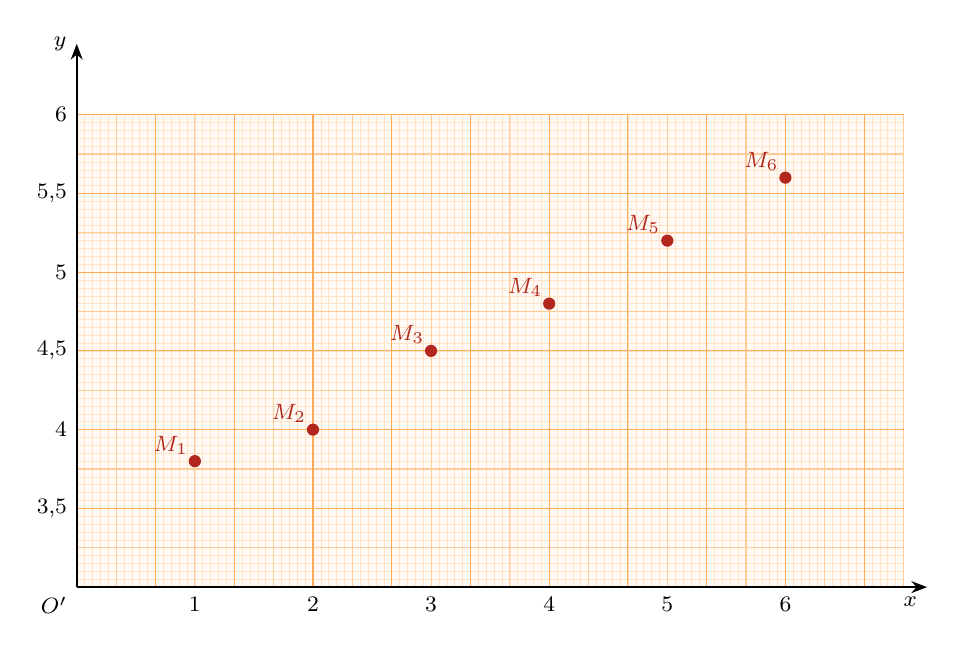
\begin{tikzpicture}[x=1.5cm,y=2cm,font=\footnotesize]
\Paper{10.5cm}{6cm}
\draw[-{Stealth[length=2mm]},thick] (0,0)--(7.2,0) node[below left]{$x$};
\draw[-{Stealth[length=2mm]},thick] (0,0)--(0,3.45) node[left]{$y$};
\node[below left] at (0,0){$O'$};
\foreach \t in {1,...,6} \node[below] at (\t,0){$\t$};
\foreach \t/\l in {0.5/3{,}5,1/4,1.5/4{,}5,2/5,2.5/5{,}5,3/6} \node[left] at (0,\t){$\l$};
\begin{scope}[shift={(0,-3)}]
\foreach \a/\b in {1/3.8,2/4,3/4.5,4/4.8,5/5.2,6/5.6} {\Pt{(\a,\b)}\node[above left=-1pt,cThm] at (\a,\b){$M_{\a}$};}
\end{scope}
\end{tikzpicture}
\end{FIG}
النقط تقريبًا على استقامة واحدة: نفكر في \textbf{تعديل خطي} (نبحث عن مستقيم يمر بالقرب من النقط).
\end{mithal}

\begin{molahada}
\begin{itemize}
\item إذا كانت النقط \textbf{متقاربة من مستقيم} نقوم بتعديل خطي $y=ax+b$.
\item إذا كان شكل السحابة \textbf{منحنيًا} (نمو سريع يشبه $e^{x}$) نقوم بتغيير متغير مثل $z=\ln y$ (الفقرة 7).
\end{itemize}
\end{molahada}

\section{النقطة المتوسطة}
\begin{tarif}
النقطة المتوسطة لسحابة النقط هي النقطة $G(\overline{x};\overline{y})$ حيث:
\[\overline{x}=\frac{x_1+x_2+\cdots+x_n}{n}=\frac{1}{n}\sum_{i=1}^{n}x_i
\qquad;\qquad
\overline{y}=\frac{1}{n}\sum_{i=1}^{n}y_i\]
\end{tarif}

\begin{mithal}
في المثال المرجعي: $\overline{x}=\dfrac{1+2+3+4+5+6}{6}=\dfrac{21}{6}=3,5$ \ و\ $\overline{y}=\dfrac{3,8+4+4,5+4,8+5,2+5,6}{6}=\dfrac{27,9}{6}=4,65$.

إذن: \bx{G(3,5\,;\,4,65)}.
\end{mithal}

\section{التعديل الخطي بطريقة ماير}
\begin{tariqa}[طريقة ماير]
\begin{enumerate}[label=\textbf{\arabic*.}]
\item نرتب النقط حسب $x_i$ تصاعديًا، ثم نقسم السحابة إلى \textbf{مجموعتين} لهما نفس عدد النقط (أو يختلفان بنقطة واحدة إذا كان $n$ فرديًا).
\item نحسب النقطتين المتوسطتين $G_1$ للمجموعة الأولى و$G_2$ للمجموعة الثانية.
\item \textbf{مستقيم ماير} هو المستقيم $(G_1G_2)$: معامل توجيهه $a=\dfrac{y_{G_2}-y_{G_1}}{x_{G_2}-x_{G_1}}$، ثم $b$ من شرط مروره بـ $G_1$.
\end{enumerate}
\end{tariqa}

\begin{khassia}
مستقيم ماير $(G_1G_2)$ يشمل دائمًا النقطة المتوسطة $G$ للسحابة كلها (عندما يكون للمجموعتين نفس عدد النقط).
\end{khassia}

\begin{mithal}[مستقيم ماير للمثال المرجعي]
المجموعة الأولى: $M_1,M_2,M_3$؛ المجموعة الثانية: $M_4,M_5,M_6$.
\begin{align*}
x_{G_1}&=\frac{1+2+3}{3}=2, & y_{G_1}&=\frac{3,8+4+4,5}{3}=4,1\\
x_{G_2}&=\frac{4+5+6}{3}=5, & y_{G_2}&=\frac{4,8+5,2+5,6}{3}=5,2
\end{align*}
إذن $G_1(2\,;4,1)$ و$G_2(5\,;5,2)$. معامل التوجيه: $a=\dfrac{5,2-4,1}{5-2}=\dfrac{1,1}{3}=\dfrac{11}{30}\approx0,367$.

$G_1\in(G_1G_2)$: $4,1=\dfrac{11}{30}\times2+b$ ومنه $b=4,1-\dfrac{22}{30}=\dfrac{101}{30}\approx3,367$.
\[\bx{(G_1G_2):\ y=\frac{11}{30}x+\frac{101}{30}\approx0,367x+3,367}\]
\textbf{تحقق:} $\dfrac{11}{30}\times3,5+\dfrac{101}{30}=\dfrac{38,5+101}{30}=\dfrac{139,5}{30}=4,65=\overline{y}$، إذن $G\in(G_1G_2)$ \ok.
\end{mithal}

\begin{FIG}
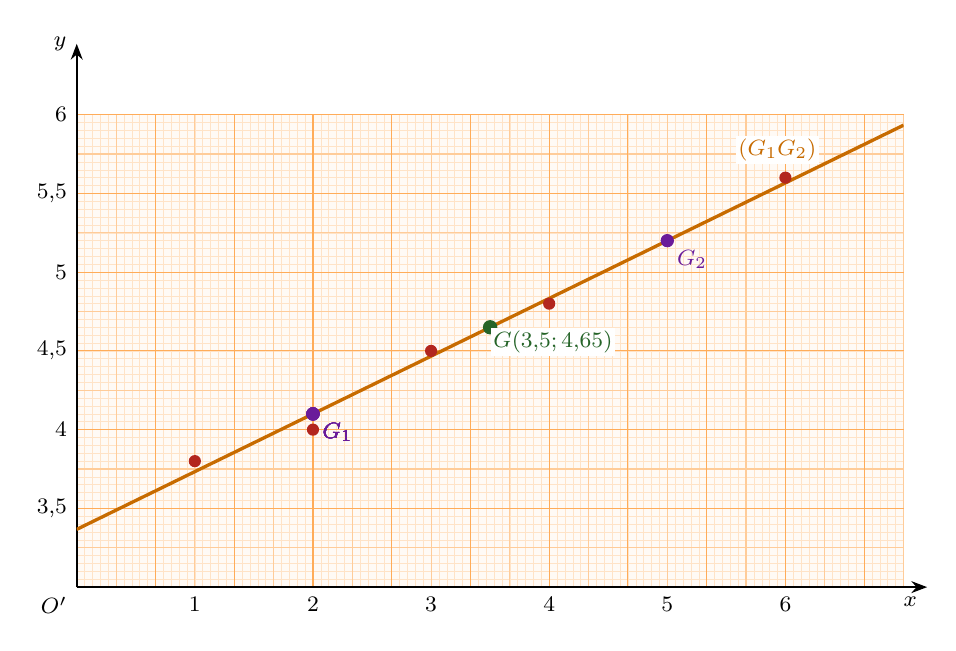
\begin{tikzpicture}[x=1.5cm,y=2cm,font=\footnotesize]
\Paper{10.5cm}{6cm}
\draw[-{Stealth[length=2mm]},thick] (0,0)--(7.2,0) node[below left]{$x$};
\draw[-{Stealth[length=2mm]},thick] (0,0)--(0,3.45) node[left]{$y$};
\node[below left] at (0,0){$O'$};
\foreach \t in {1,...,6} \node[below] at (\t,0){$\t$};
\foreach \t/\l in {0.5/3{,}5,1/4,1.5/4{,}5,2/5,2.5/5{,}5,3/6} \node[left] at (0,\t){$\l$};
\begin{scope}[shift={(0,-3)}]
\clip (0,3) rectangle (7,6);
\draw[cEx,very thick] (0,101/30)--(7,11/30*7+101/30) node[pos=0.9,above left,fill=white,inner sep=1pt]{$(G_1G_2)$};
\foreach \a/\b in {1/3.8,2/4,3/4.5,4/4.8,5/5.2,6/5.6} \Pt{(\a,\b)}
\fill[cMeth] (2,4.1) circle (2.4pt) node[below right]{$G_1$};
\fill[cMeth] (5,5.2) circle (2.4pt) node[below right]{$G_2$};
\fill[cRem!80!black] (3.5,4.65) circle (2.6pt) node[below right,fill=white,inner sep=1pt]{$G(3{,}5;4{,}65)$};
\end{scope}
\end{tikzpicture}
\end{FIG}

\begin{molahada}[$n$ فردي]
إذا كان $n$ فرديًا يحدد النص المجموعتين (مثلا $3$ نقط ثم $4$ نقط)؛ عندئذ قد لا يشمل $(G_1G_2)$ النقطة $G$ تمامًا.
\end{molahada}

\section{مستقيم تعديل بالرسم أو مستقيم تعديل معطى}
\begin{tariqa}[تعديل بياني (بالعين)]
\begin{enumerate}[label=\textbf{\arabic*.}]
\item نعلّم النقطة المتوسطة $G$ ثم نرسم مستقيمًا يشمل $G$ ويمر بالقرب من النقط، ويترك تقريبًا نفس عدد النقط من كل جهة.
\item نقرأ إحداثيي نقطة ثانية $A$ من هذا المستقيم (غالبًا نقطة من السحابة يمر بها)، ثم نحسب معادلته $y=ax+b$ من النقطتين $G$ و$A$.
\end{enumerate}
\end{tariqa}

\begin{tariqa}[مستقيم تعديل معطى في النص]
إذا أعطى النص مستقيمًا $(D):\ y=ax+b$ وطلب «تحقق» أو «بيّن أنه مستقيم تعديل»: نتحقق أن $G\in(D)$ أي $\overline{y}=a\overline{x}+b$ (بتقريب التدوير)، ثم نرسمه بنقطتين ($G$ ونقطة أخرى). يمكن قراءة معادلة مستقيم التعديل أيضًا \textbf{بالآلة الحاسبة} (الوضع \textbf{STAT}، النمط $A+BX$) للتحقق.
\end{tariqa}

\begin{mithal}[المثال المرجعي]
نقبل المستقيم $(D):\ y=0,37x+3,355$ مستقيم تعديل. \ $0,37\times3,5+3,355=1,295+3,355=4,65=\overline{y}$، إذن \bx{G\in(D)} \ok.

لرسمه: $G(3,5;4,65)$ والنقطة $(1\,;3,725)$ لأن $0,37\times1+3,355=3,725$. المستقيمان $(D)$ و$(G_1G_2)$ متقاربان جدًا (معامل التوجيه $0,37$ مقابل $\frac{11}{30}\approx0,367$).
\end{mithal}

\section{التقدير (التنبؤ)}
\begin{tariqa}[استعمال معادلة التعديل $y=ax+b$]
\begin{enumerate}[label=\textbf{\arabic*.}]
\item \textbf{تقدير $y$ لقيمة معطاة لـ $x$:} نحسب الرتبة $x$ الموافقة (ننتبه للعلاقة بين السنة والرتبة) ثم نعوض: $y=ax+b$.
\item \textbf{إيجاد $x$ ليبلغ $y$ قيمة $y_0$:} نحل $ax+b=y_0$ (أو المتراجحة $ax+b\ge y_0$)، ثم نأخذ أصغر رتبة طبيعية مناسبة ونرجع إلى السنة.
\end{enumerate}
\end{tariqa}

\begin{mithal}[المثال المرجعي (بمستقيم ماير)]
\textbf{1.} تقدير إنتاج سنة 2009: رتبتها $x=2009-1999=10$، ومنه $y=\dfrac{11}{30}\times10+\dfrac{101}{30}=\dfrac{211}{30}\approx7,03$ مليون طن.

إذا كان هدف المعمل بلوغ $7,3$ مليون طن سنة 2009: $7,03<7,3$ إذن \bxt{الهدف لا يتحقق حسب هذا التعديل}.

\textbf{2.} متى يتجاوز الإنتاج $7,3$ مليون طن؟ \ $\dfrac{11}{30}x+\dfrac{101}{30}\ge7,3 \iff 11x+101\ge219 \iff x\ge\dfrac{118}{11}\approx10,73$، أي $x=11$ والسنة $1999+11=2010$.
\end{mithal}

\begin{molahada}
التقدير خارج مجال المعطيات (الاستكمال) يفترض أن الوتيرة تبقى نفسها؛ لذا نكتب «حسب هذا التعديل» أو «إذا بقيت الوتيرة نفسها».
\end{molahada}

\section{تغيير المتغير: التعديل الأسي}
\begin{tariqa}[الوضع $z=\ln y$ \ (حيث $y_i>0$)]
\begin{enumerate}[label=\textbf{\arabic*.}]
\item عندما تكون السحابة $(x_i;y_i)$ منحنية (نمو سريع)، نضع $z_i=\ln y_i$ وندور كما يطلب النص.
\item ندرس السلسلة $(x_i;z_i)$: نحسب $G(\overline{x};\overline{z})$ ثم مستقيم تعديل $z=ax+b$ (طريقة ماير، أو المستقيم المعطى في النص بعد التحقق أنه يشمل $G$).
\item نرجع إلى $y$:
\[z=ax+b\iff\ln y=ax+b\iff y=e^{ax+b}\iff\bx{y=e^{b}\,e^{ax}=k\,q^{x}}\]
حيث $k=e^{b}$ و$q=e^{a}$.
\end{enumerate}
\end{tariqa}

\origNeedspace{18\baselineskip}\begin{mithal}[تعديل أسي -- مثال محلول بطريقة ماير]
تطور عدد مشتركي خدمة (بالآلاف) $y_i$ حسب رتبة الشهر $x_i$:
\begin{center}
\begin{tabular}{|C|c|c|c|c|c|c|}\hline
\rowcolor{cSec!12} $x_i$ & $0$ & $1$ & $2$ & $3$ & $4$ & $5$\\\hline
$y_i$ & $2$ & $3,1$ & $4,4$ & $6,7$ & $9,9$ & $14,8$\\\hline
$z_i=\ln y_i$ & $0,69$ & $1,13$ & $1,48$ & $1,90$ & $2,29$ & $2,69$\\\hline
\end{tabular}
\end{center}
($z_i$ مدورة إلى $10^{-2}$.) المجموعة الأولى $x_i\in\{0;1;2\}$ والثانية $x_i\in\{3;4;5\}$:
\[G_1\left(1\,;\,\frac{0,69+1,13+1,48}{3}\right)=G_1(1\,;1,1)\qquad G_2\left(4\,;\,\frac{1,90+2,29+2,69}{3}\right)\approx G_2(4\,;2,2933)\]
$a=\dfrac{2,2933-1,1}{4-1}\approx0,3978\approx0,40$ \ ؛ \ $b=1,1-0,3978\times1\approx0,7022\approx0,70$، \ إذن \ $z=0,40x+0,70$.

\textbf{الرجوع إلى $y$:} $\ln y=0,40x+0,70$ ومنه $y=e^{0,70}\times e^{0,40x}$؛ مع $e^{0,70}\approx2,01$ و$e^{0,40}\approx1,49$:
\[\bx{y\approx2,01\times(1,49)^{x}}\]
\textbf{تقدير} الشهر ذي الرتبة $6$: $y=e^{0,70+0,40\times6}=e^{3,1}\approx22,2$ ألف مشترك.
\end{mithal}

\begin{molahada}
\begin{itemize}
\item يمكن طلب وضع آخر مثل $z=\ln(y-c)$ أو $t=\ln x$: نطبق نفس الخطوات ثم نرجع إلى المتغير الأصلي.
\item للتنبؤ نستعمل الصيغة الأسية (لا المستقيم $z=ax+b$ مباشرة إلا إذا رجعنا بـ $y=e^{z}$).
\end{itemize}
\end{molahada}

%================================================================
\origNeedspace{26\baselineskip}\section{تمارين محلولة من نمط البكالوريا}
\begin{tmr}
يمثل الجدول ضغط الدم $y_i$ بدلالة السن $x_i$ لعينة من الرجال:
\begin{center}
\begin{tabular}{|C|c|c|c|c|c|c|c|}\hline
\rowcolor{cSec!12} السن $x_i$ & $35$ & $40$ & $45$ & $50$ & $55$ & $60$ & $65$\\\hline
ضغط الدم $y_i$ & $12,2$ & $12,4$ & $12,5$ & $13$ & $13,3$ & $13,6$ & $14$\\\hline
\end{tabular}
\end{center}
\QQ{1} مثّل سحابة النقط $M_i(x_i;y_i)$ في معلم متعامد مبدؤه $O'(30;11)$ وبحيث: $1cm$ لكل 5 سنوات على محور الفواصل و$2cm$ لكل وحدة على محور التراتيب.
\QQ{2} عيّن إحداثيي النقطة المتوسطة $G$ ثم مثلها.
\QQ{3} نقبل أن المستقيم $(D):\ y=0,06x+10$ مستقيم تعديل لهذه السحابة. تحقق أن $G\in(D)$ ثم ارسمه.
\QQ{4} رجل عمره 70 سنة وضغط دمه $15,2$. هل هذا معقول حسب هذا التعديل؟ علّل.
\end{tmr}
\begin{hal}
\QQ{1} السحابة (المبدأ $O'(30;11)$ ، $1cm\leftrightarrow5$ سنوات، $2cm\leftrightarrow1$):
\begin{FIG}
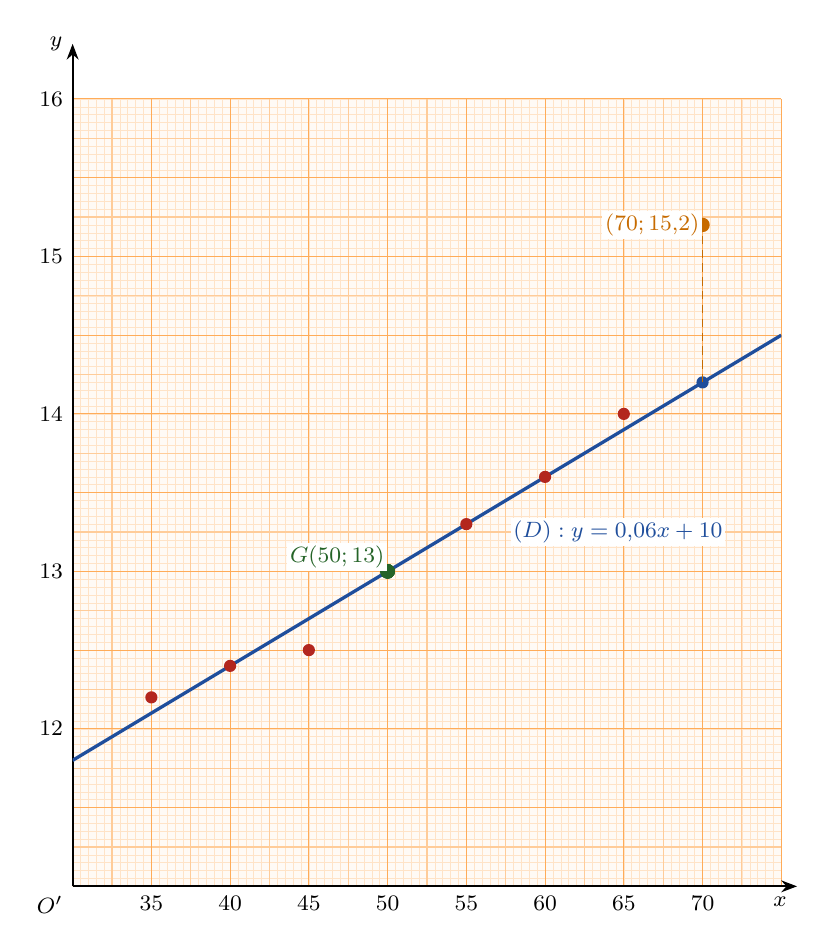
\begin{tikzpicture}[x=0.2cm,y=2cm,font=\footnotesize]
\Paper{9cm}{10cm}
\draw[-{Stealth[length=2mm]},thick] (0,0)--(46,0) node[below left]{$x$};
\draw[-{Stealth[length=2mm]},thick] (0,0)--(0,5.35) node[left]{$y$};
\node[below left] at (0,0){$O'$};
\foreach \t in {35,40,...,70} \node[below] at (\t-30,0){$\t$};
\foreach \t in {12,13,14,15,16} \node[left] at (0,\t-11){$\t$};
\begin{scope}[shift={(-30,-11)}]
\clip (30,11) rectangle (75,16);
\draw[cDef,very thick] (30,0.06*30+10)--(75,0.06*75+10) node[pos=0.6,below right=4pt,fill=white,inner sep=1pt]{$(D):y=0{,}06x+10$};
\foreach \a/\b in {35/12.2,40/12.4,45/12.5,50/13,55/13.3,60/13.6,65/14} \Pt{(\a,\b)}
\fill[cRem!80!black] (50,13) circle (2.6pt) node[above left,fill=white,inner sep=1pt]{$G(50;13)$};
\fill[cEx] (70,15.2) circle (2.6pt) node[left,fill=white,inner sep=1pt]{$(70;15{,}2)$};
\fill[cDef] (70,14.2) circle (2.2pt);
\draw[cEx,densely dashed] (70,14.2)--(70,15.2);
\end{scope}
\end{tikzpicture}
\end{FIG}
\QQ{2} $\overline{x}=\dfrac{350}{7}=50$ \ و\ $\overline{y}=\dfrac{91}{7}=13$، إذن \bx{G(50\,;13)}.

\QQ{3} $0,06\times50+10=3+10=13=\overline{y}$، إذن \bx{G\in(D)} \ok. (الآلة الحاسبة في الوضع \textbf{STAT} تعطي معاملًا قريبًا: $a\approx0,061$.)

للرسم: النقطتان $G(50;13)$ و$(30\,;11,8)$ لأن $0,06\times30+10=11,8$.

\QQ{4} من أجل $x=70$: $y=0,06\times70+10=14,2$. \quad الضغط المقدر $14,2$ والضغط الحقيقي $15,2>14,2$ (بفارق $1$ وهو كبير مقارنة بتشتت النقط حول $(D)$).

إذن \bxt{ضغط دمه غير معقول حسب هذا التعديل (مرتفع)}.
\end{hal}

\begin{tmr}
يعطي الجدول تطور عدد مستعملي الهاتف النقال $y_i$ في مدينة، حيث $x_i$ رتبة السنة ($x_i=1$ توافق سنة 2006):
\begin{center}
\setlength{\tabcolsep}{4pt}
\begin{tabular}{|C|c|c|c|c|c|c|c|}\hline
\rowcolor{cSec!12} السنة & $2006$ & $2007$ & $2008$ & $2009$ & $2010$ & $2011$ & $2012$\\\hline
رتبة السنة $x_i$ & $1$ & $2$ & $3$ & $4$ & $5$ & $6$ & $7$\\\hline
عدد المستعملين $y_i$ & $21400$ & $32400$ & $48000$ & $75600$ & $121200$ & $207000$ & $280000$\\\hline
\end{tabular}
\end{center}
\QQ{1}
\begin{sq}
\qa مثّل سحابة النقط $M_i(x_i;y_i)$ ($1cm$ لكل سنة، $0,5cm$ لكل $20000$ مستعمل).
\qb هل يمكن تسوية هذه السحابة بتعديل خطي؟ برر.
\end{sq}
\QQ{2} نضع $z_i=\ln y_i$ (تدور النتائج إلى $10^{-2}$).
\begin{sq}
\qa أنشئ جدول السلسلة $(x_i;z_i)$ ومثّل سحابتها في معلم مبدؤه $O'(0;9)$ ($1cm$ لكل سنة، $2cm$ لكل وحدة).
\qb عيّن إحداثيي النقطة المتوسطة $G$ لهذه السحابة.
\qc نقبل المستقيم $(\Delta):\ z=0,44x+9,51$ مستقيم تعديل للسلسلة $(x_i;z_i)$. تحقق أنه يشمل $G$ (بتقريب $10^{-2}$) ثم ارسمه.
\end{sq}
\QQ{3}
\begin{sq}
\qa تحقق أن $y=k\,e^{0,44x}$ حيث $k$ عدد حقيقي يطلب تعيينه (يدور إلى الوحدة).
\qb بفرض أن الوتيرة نفسها، قدّر عدد المستعملين سنة 2014.
\qc ابتداءً من أي سنة يتجاوز عدد المستعملين مليون مستعمل؟
\end{sq}
\end{tmr}
\begin{hal}
\QQ{1}\pa السحابة (التراتيب بالمستعملين):
\begin{FIG}
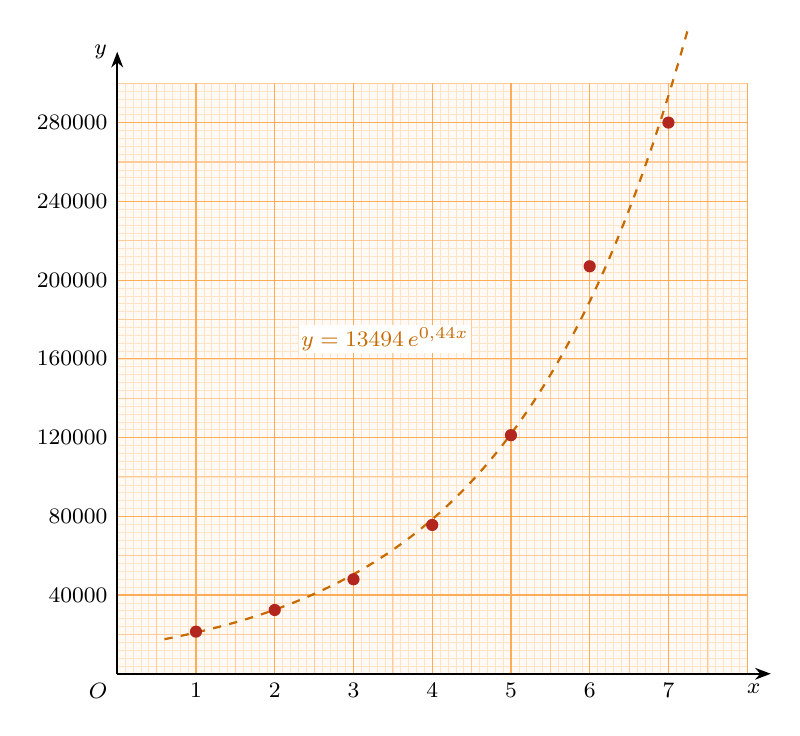
\begin{tikzpicture}[x=1cm,y=0.5cm,font=\footnotesize]
\Paper{8cm}{7.5cm}
\draw[-{Stealth[length=2mm]},thick] (0,0)--(8.3,0) node[below left]{$x$};
\draw[-{Stealth[length=2mm]},thick] (0,0)--(0,15.8) node[left]{$y$};
\node[below left] at (0,0){$O$};
\foreach \t in {1,...,7} \node[below] at (\t,0){$\t$};
\foreach \t/\l in {2/40000,4/80000,6/120000,8/160000,10/200000,12/240000,14/280000} \node[left] at (0,\t){$\l$};
\draw[cEx,thick,dashed,domain=0.6:7.25,samples=60] plot (\x,{0.6747*exp(0.44*\x)});
\foreach \a/\b in {1/1.07,2/1.62,3/2.4,4/3.78,5/6.06,6/10.35,7/14} \Pt{(\a,\b)}
\node[cEx,fill=white,inner sep=1pt] at (3.4,8.5){$y=13494\,e^{0{,}44x}$};
\end{tikzpicture}
\end{FIG}
\pb \textbf{لا}: النقط ليست قريبة من مستقيم، السحابة منحنية (نمو سريع من نوع أسي)، لذا التعديل الخطي غير ملائم.

\QQ{2}\pa قيم $z_i$ ($n=7$):
\begin{center}
\setlength{\tabcolsep}{3pt}\small
\begin{tabular}{|C|c|c|c|c|c|c|c|>{\columncolor{cRem!10}}C|}\hline
\rowcolor{cSec!12} $x_i$ & $1$ & $2$ & $3$ & $4$ & $5$ & $6$ & $7$ & المجموع: $28$\\\hline
$z_i=\ln y_i$ & $9,97$ & $10,39$ & $10,78$ & $11,23$ & $11,71$ & $12,24$ & $12,54$ & $78,86$\\\hline
\end{tabular}
\end{center}
\begin{FIG}
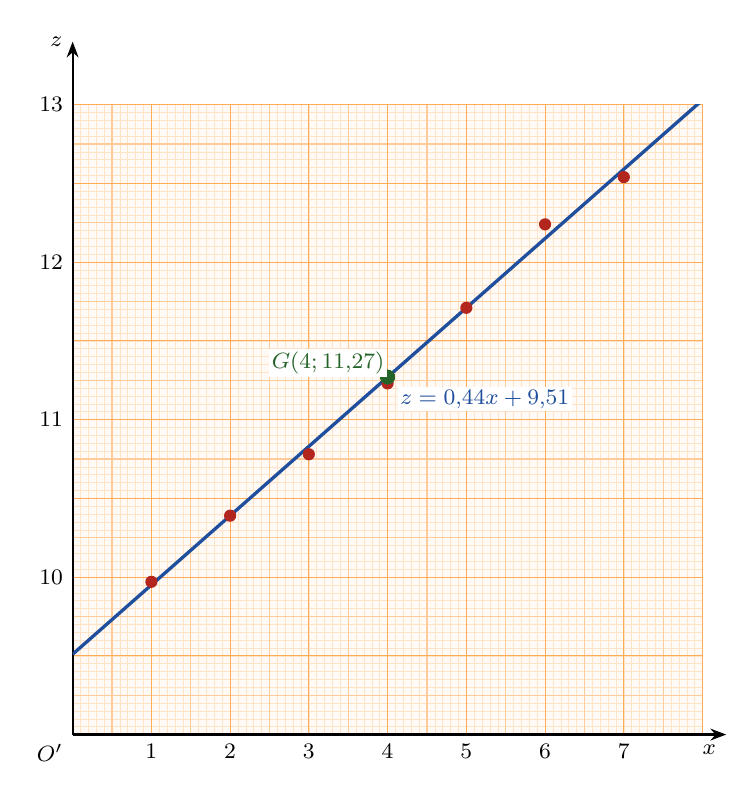
\begin{tikzpicture}[x=1cm,y=2cm,font=\footnotesize]
\Paper{8cm}{8cm}
\draw[-{Stealth[length=2mm]},thick] (0,0)--(8.3,0) node[below left]{$x$};
\draw[-{Stealth[length=2mm]},thick] (0,0)--(0,4.4) node[left]{$z$};
\node[below left] at (0,0){$O'$};
\foreach \t in {1,...,7} \node[below] at (\t,0){$\t$};
\foreach \t in {10,11,12,13} \node[left] at (0,\t-9){$\t$};
\begin{scope}[shift={(0,-9)}]
\clip (0,9) rectangle (8,13);
\draw[cDef,very thick] (0,9.51)--(8,0.44*8+9.51) node[pos=0.5,below right=3pt,fill=white,inner sep=1pt]{$z=0{,}44x+9{,}51$};
\foreach \a/\b in {1/9.97,2/10.39,3/10.78,4/11.23,5/11.71,6/12.24,7/12.54} \Pt{(\a,\b)}
\fill[cRem!80!black] (4,11.27) circle (2.6pt) node[above left,fill=white,inner sep=1pt]{$G(4;11{,}27)$};
\end{scope}
\end{tikzpicture}
\end{FIG}
\pb $\overline{x}=\dfrac{28}{7}=4$ \ و\ $\overline{z}=\dfrac{78,86}{7}\approx11,2657\approx11,27$، إذن \bx{G(4\,;11,27)}.

\pc $0,44\times4+9,51=1,76+9,51=11,27=\overline{z}$ (بتقريب $10^{-2}$)، إذن \bx{G\in(\Delta)} \ok. للرسم: $G(4;11,27)$ والنقطة $(0\,;9,51)$.

\QQ{3}\pa $\ln y=0,44x+9,51$ ومنه $y=e^{9,51}\times e^{0,44x}$. \ $k=e^{9,51}\approx13493,99$، إذن \bx{y=13494\,e^{0,44x}}.

\pb سنة 2014 توافق $x=2014-2005=9$: \ $y=13494\,e^{0,44\times9}=13494\,e^{3,96}\approx707859$.

حسب هذا التعديل: حوالي \bxt{$707\,859$ مستعملًا سنة 2014}.

\pc $13494\,e^{0,44x}>10^{6}\iff e^{9,51+0,44x}>10^{6}\iff9,51+0,44x>\ln10^{6}\approx13,8155\iff x>\dfrac{4,3055}{0,44}\approx9,79$.

أصغر رتبة: $x=10$، أي السنة $2005+10=2015$.
\end{hal}



%================================================================
\section{أخطاء شائعة}
\begin{BOX}{cThm}{تجنّب هذه الأخطاء}
\begin{enumerate}[label=\textbf{\arabic*.}]
\item نسيان القسمة على $n$ في حساب $\overline{x}$ و$\overline{y}$.
\item الخلط بين \textbf{السنة} و\textbf{رتبتها} عند التقدير: نحول السنة إلى رتبة قبل التعويض، ثم نرجع إلى السنة في الجواب.
\item التدوير المبكر لإحداثيات $G_1$ و$G_2$: يغير قيمة $a$. ندور النتيجة النهائية فقط.
\item حساب معامل التوجيه بالمقلوب $\dfrac{x_{G_2}-x_{G_1}}{y_{G_2}-y_{G_1}}$؛ الصحيح $a=\dfrac{y_{G_2}-y_{G_1}}{x_{G_2}-x_{G_1}}$.
\item عدم احترام المبدأ $O'$ والوحدات المعطاة في رسم السحابة، أو تدريج المحور من $0$ بدل بداية المبدأ.
\item في طريقة ماير: تقسيم السحابة دون ترتيب $x_i$ تصاعديًا، أو مجموعتان غير متوازنتين.
\item في التعديل الأسي: الخطأ $y=e^{a}x+e^{b}$؛ الصحيح $y=e^{b}e^{ax}$. واستعمال $z=ax+b$ مباشرة للتنبؤ بقيمة $y$.
\item قبول مستقيم تعديل معطى دون التحقق أنه يشمل $G$، أو رسم مستقيم بياني لا يمر بـ $G$.
\item إجابة سؤال «من أي سنة» برتبة غير طبيعية: نأخذ أصغر عدد طبيعي يحقق المتراجحة.
\end{enumerate}
\end{BOX}

\section{خلاصة الطرائق}
\begin{BOX}{cMeth}{الطريقة حسب المطلوب}
\begin{center}
\renewcommand{\arraystretch}{1.35}
\begin{tabular}{|p{0.62\textwidth}|p{0.3\textwidth}|}\hline
\rowcolor{cSec!12} \textbf{الطريقة} & \textbf{المطلوب}\\\hline
نحترم المبدأ $O'(x_0;y_0)$ والوحدات، ونعلّم النقط $M_i(x_i;y_i)$. & تمثيل سحابة النقط\\\hline
$\overline{x}=\frac1n\sum x_i$ ، $\overline{y}=\frac1n\sum y_i$. & النقطة المتوسطة $G$\\\hline
نرتب حسب $x_i$، نقسم إلى مجموعتين، نحسب $G_1$ و$G_2$، ثم معادلة $(G_1G_2)$ (يشمل $G$). & مستقيم ماير\\\hline
نرسم مستقيمًا يشمل $G$ ويترك نفس عدد النقط تقريبًا من كل جهة، ثم معادلته من $G$ ونقطة ثانية. & تعديل بياني\\\hline
نتحقق أن $\overline{y}=a\overline{x}+b$ (أي $G\in(D)$)، ثم نرسمه بنقطتين. & مستقيم تعديل معطى\\\hline
نحول السنة إلى رتبة ثم نعوض في $y=ax+b$؛ أو نحل $ax+b\ge y_0$ ونأخذ أصغر رتبة طبيعية. & التقدير (التنبؤ)\\\hline
$z=\ln y$ ، ثم $z=ax+b$ ، ثم $y=e^{b}e^{ax}=k\,q^{x}$. & سحابة منحنية: تعديل أسي\\\hline
\end{tabular}
\end{center}
\end{BOX}
\end{document}
